\documentclass[11pt]{article}
\usepackage[margin=1in]{geometry}
\usepackage{amsmath,amssymb,mathtools,bm}
\usepackage{booktabs}
\usepackage{microtype}
\usepackage{graphicx}
\usepackage{enumitem}
\usepackage{hyperref}
\usepackage{cleveref}
\usepackage{xcolor}
\usepackage{caption}
\usepackage{subcaption}
\usepackage{float}
\usepackage{siunitx}
\usepackage{setspace}
\usepackage{authblk}

\hypersetup{colorlinks=true,linkcolor=blue,citecolor=blue,urlcolor=blue}
\setlength{\parskip}{0.45em}
\setlength{\parindent}{0pt}
\onehalfspacing

\newcommand{\Rzero}{\mathcal R_0}
\newcommand{\rhoeps}{\rho}
\newcommand{\hth}{h_\theta}
\newcommand{\xf}{x_f}
\newcommand{\xs}{x_*}
\newcommand{\yin}{y_{\rm BL}}
\newcommand{\xin}{x_{\rm in}}
\newcommand{\Cth}{C_\theta}
\newcommand{\Dth}{D_\theta}
\newcommand{\Ath}{A_\theta}
\newcommand{\dAf}{\Delta A_f}
\newcommand{\dd}{\,\mathrm d}
\newcommand{\BI}{\mathrm{BI}}

\title{Epidemic Burnout under General Susceptible Recruitment}
\author{Draft manuscript}
\date{September 2026}

\begin{document}
\maketitle

\begin{abstract}
[[JD: Would be good to get a bit more motivation in the abstract]]
[[JD: If we are going to use authordate style (
Parsons et al. approximated epidemic burnout after a major epidemic wave by matching a deterministic epidemic trajectory to a stochastic branching process at low prevalence. Existing asymptotic burnout theory for the susceptible--infectious--recovered model with vital dynamics assumes linear susceptible replenishment. Motivated by the possibility of density-dependent recruitment, particularly in ecological host populations, we replace the linear term by the one-parameter family
\(
\hth(x)=(1-x)x^\theta,\qquad 0\leq \theta\leq 1,
\)
[[JD: Maybe don't need equation here, just say we interpolate]].
[[JD: initial instead of leading below (and elsewhere in this context)]]
which interpolates continuously between linear and logistic replenishment. In the limit of slow susceptible recruitment, the leading trajectory of the first epidemic wave is unchanged by the recruitment law. The effect of \(\theta\) appears instead in the post-wave decline, where small corrections to the susceptible fraction can strongly affect how deeply infection falls before susceptible replenishment permits recovery. We derive first- and second-order asymptotic approximations for this post-epidemic trajectory and for the state at which infection enters the low-prevalence regime. We then use these deterministic approximations as input to Kendall's time-inhomogeneous branching-process calculation to obtain the probability of extinction during the first epidemic trough. Matching the deterministic and stochastic descriptions in their common regime of validity yields a leading-order prediction for the trough depth and burnout probability that does not depend on an arbitrarily chosen matching threshold. 
[[JD: Bolker commented here, should discuss. I like the idea of selling this finding, but it's not clear how or where.]]
Stochastic simulations show close quantitative agreement in the separated small-\(\rhoeps\) regime. Increasing \(\theta\) can strongly suppress post-wave persistence and reorganizes the nonmonotone dependence of unconditional persistence on \(\Rzero\): over the parameter ranges examined, an existing minimum moves to larger \(\Rzero\) at small recruitment rates, while at larger recruitment rates a maximum--minimum pair is created across a \(K\)-dependent saddle-node boundary. The analysis extends the deterministic--stochastic burnout framework to a broader family of susceptible-recruitment laws and identifies both quantitative and qualitative ways in which recruitment shape modifies survival through the post-wave trough.
\end{abstract}

\section{Introduction}
Large epidemic outbreaks can end in two qualitatively different ways. Infection may remain present after the first epidemic wave and recover as susceptible hosts are replenished, or it may disappear while prevalence is still very low. The second outcome is often described as epidemic burnout. Full stochastic simulation can capture both the epidemic wave and the subsequent extinction process, but repeated simulation becomes costly when persistence probabilities must be evaluated across large parameter ranges. A useful approximation is therefore to describe the macroscopic epidemic wave deterministically and treat the low-prevalence phase stochastically.

Parsons and Earn developed uniform asymptotic phase-plane approximations for the SIR model with vital dynamics, and Parsons, Bolker, Dushoff, and Earn subsequently coupled this deterministic structure to a time-inhomogeneous branching-process calculation of first-trough burnout probability \cite{ParsonsEarn2024,ParsonsEtAl2024}. In that setting susceptible replenishment is linear. Here we ask how the same analytical framework changes when susceptible recruitment is density dependent. Such density dependence is natural in ecological population models, where recruitment may decrease as a population approaches a carrying capacity, whereas linear demographic turnover is a common approximation in standard human-disease SIR models.

We replace linear replenishment by
\[
\hth(x)=(1-x)x^\theta,\qquad 0\leq\theta\leq1.
\]
The case \(\theta=0\) recovers the standard linear model, whereas \(\theta=1\) gives logistic replenishment. This formulation allows us to study how changing the susceptible-recruitment law alters the post-wave trough and the probability of epidemic persistence.

A key simplification is that the leading trajectory of the first epidemic wave does not depend on \(\theta\). When susceptible recruitment is neglected, all models in the family follow the same epidemic orbit. The effect of the recruitment law appears in the corrections to this trajectory as the epidemic declines toward low prevalence. These corrections determine how deeply infection falls after the first wave and therefore affect the subsequent probability of burnout.

Building on the phase-plane and epidemic-burnout approximations developed in earlier work \cite{ParsonsEarn2024,ParsonsEtAl2024}, we derive the corresponding first- and second-order post-wave corrections for the generalized recruitment law, extend the existing matching and trough approximations to this setting, and use the resulting low-prevalence entry states in Kendall's time-inhomogeneous birth--death calculation to evaluate burnout and persistence probabilities.

The paper is organized as follows. Section~\ref{sec:model} introduces the generalized SIR model and formulates the post-wave burnout problem. Section~\ref{sec:phaseplane} develops the leading epidemic orbit and its first- and second-order corrections under generalized susceptible recruitment. Section~\ref{sec:matching} analyzes the post-wave low-prevalence regime and derives the matching quantities required to connect the epidemic trajectory to the stochastic calculation. Section~\ref{sec:action} reformulates this matching problem in terms of an action variable and derives finite-threshold estimates for the low-prevalence entry state. Section~\ref{sec:burnout} combines these results with Kendall's time-inhomogeneous birth--death formulation and derives the corresponding burnout and persistence approximations. Section~\ref{sec:numerics} compares the approximations with stochastic simulations and examines the effect of the recruitment-shape parameter \(\theta\). Section~\ref{sec:discussion} discusses interpretation, limitations, and possible extensions of the framework.

\section{Generalized SIR model and epidemic burnout}
\label{sec:model}
We consider the dimensionless SIR-type system
\begin{align}
\frac{\dd x}{\dd \sigma} &= \rhoeps\hth(x)-\Rzero xy,\label{eq:modelx}\\
\frac{\dd y}{\dd \sigma} &= (\Rzero x-1)y,\label{eq:modely}
\end{align}
where \(x\) is the susceptible fraction, \(y\) is the infectious fraction, \(\sigma\) is time scaled by the infectious removal rate, \(\Rzero>1\) is the basic reproduction number, and \(0<\rhoeps\ll1\) is the susceptible-recruitment rate divided by the infectious removal rate. Recruitment is
\begin{equation}
\hth(x)=(1-x)x^\theta,\qquad 0\leq\theta\leq1.
\label{eq:hth}
\end{equation}
For \(\theta=0\), \(\hth(x)=1-x\) is the standard linear replenishment law. For \(\theta=1\), \(\hth(x)=x(1-x)\) is logistic replenishment. At small susceptible density,
\[
\hth(x)\sim x^\theta,\qquad x\downarrow0,
\]
so \(\theta\) controls the low-density dependence of recruitment.

The infectious growth threshold is
\begin{equation}
\xs=\frac{1}{\Rzero}.
\label{eq:xstar}
\end{equation}
The endemic equilibrium has susceptible fraction \(\xs\) and infectious fraction
\begin{equation}
y_*=\rhoeps\hth(\xs)=\rhoeps(\Rzero-1)\Rzero^{-(1+\theta)}.
\label{eq:ystar}
\end{equation}
Let \(K\) denote the characteristic host population size.

Conditional on a successful initial invasion, the first epidemic wave can be described deterministically while prevalence remains macroscopic. As prevalence declines after the wave, however, the expected number of infectives may become sufficiently small that stochastic extinction is no longer negligible. The analysis below focuses on how the recruitment law modifies the post-wave trajectory and, through it, the probability that infection disappears during the first epidemic trough.

Throughout the main derivation we consider
\begin{equation}
\rhoeps\to0,\qquad \Rzero>1\ \text{fixed},\qquad K\ \text{large}.
\label{eq:regime}
\end{equation}
The near-threshold regime \(\Rzero\downarrow1\) requires separate treatment because the scale separation underlying the post-wave asymptotics becomes nonuniform.

\section{Phase-plane asymptotics under generalized susceptible recruitment}
\label{sec:phaseplane}
\subsection{Universal leading epidemic geometry}
Setting \(\rhoeps=0\) in \cref{eq:modelx,eq:modely} gives
\[
\frac{\dd y}{\dd x}=\frac{1}{\Rzero x}-1.
\]
Starting from a naive invasion near \((x,y)=(1,0)\), the leading first-wave orbit is
\begin{equation}
F(x)=1-x+\frac{1}{\Rzero}\log x,\qquad y=F(x).
\label{eq:F}
\end{equation}
The epidemic peak occurs at \(x=\xs\). The nontrivial post-wave zero \(\xf\in(0,\xs)\) is defined by
\begin{equation}
F(\xf)=0,
\qquad
\xf=-\frac{1}{\Rzero}W_0(-\Rzero e^{-\Rzero}),
\label{eq:xf}
\end{equation}
where \(W_0\) is the principal Lambert--\(W\) branch.

The point \(\xf\) anchors the singular matching, but it cannot simply be substituted for the finite-\(\rhoeps\) entry state. The later stochastic calculation contains an action scaled by \(1/\rhoeps\), so a displacement that vanishes algebraically as \(\rhoeps\to0\) can still change the burnout probability at leading exponential order. We therefore require a controlled expansion of the trajectory near \(\xf\).

\subsection{Exact phase plane and direct perturbation hierarchy}
The exact phase-plane equation is
\begin{equation}
\frac{\dd y}{\dd x}=
\frac{(\Rzero x-1)y}{\rhoeps\hth(x)-\Rzero xy}.
\label{eq:phaseplane}
\end{equation}
In the first-wave outer region, write
\begin{equation}
y=F(x)+\rhoeps Y_1(x)+\rhoeps^2Y_2(x)+O(\rhoeps^3).
\label{eq:outerexp}
\end{equation}
Substitution into \cref{eq:phaseplane} gives the sequential coefficient equations
\begin{align}
Y_1'(x)&=-\frac{\hth(x)(\Rzero x-1)}{\Rzero^2x^2F(x)},
&Y_1(1)&=0,
\label{eq:Y1prime}\\
Y_2'(x)&=\frac{\hth(x)(\Rzero x-1)}{\Rzero^2x^2F(x)^2}
\left[Y_1(x)-\frac{\hth(x)}{\Rzero x}\right],
&Y_2(1)&=0.
\label{eq:Y2prime}
\end{align}
The apparent singularities at \(x=1\) are removable. Thus the recruitment extension leaves the leading epidemic orbit unchanged and enters through one-dimensional coefficient equations at successive orders.

An equivalent bookkeeping device uses the zero-recruitment first integral
\[
H=x+y-\frac{1}{\Rzero}\log x.
\]
Along the full system,
\[
\frac{\dd H}{\dd\sigma}=\rhoeps\hth(x)\left(1-\frac{1}{\Rzero x}\right).
\]
Expanding \(H=1+\rhoeps H_1+\rhoeps^2H_2+\cdots\) reproduces \(H_1=Y_1\) and \(H_2=Y_2\). We use the direct phase-plane representation below because it makes the singular matching near \(\xf\) explicit.

\section{Singular matching near the post-epidemic state}
\label{sec:matching}
\subsection{First-order singularity and the matching constant \(\Cth\)}
Define
\begin{equation}
\widetilde a_\theta=\frac{\hth(\xf)}{\xf}.
\label{eq:atilde}
\end{equation}
Since
\[
F'(\xf)=\frac{\xs-\xf}{\xf}>0,
\]
the first-order outer correction develops a logarithmic singularity. It is convenient to introduce
\begin{equation}
G_\theta(x)=\Rzero Y_1(x),
\qquad
G_\theta'(x)=\frac{(\xs-x)\hth(x)}{x^2F(x)}.
\label{eq:Gtheta}
\end{equation}
As \(x\downarrow\xf\),
\[
G_\theta'(x)\sim\frac{\widetilde a_\theta}{x-\xf}.
\]
The corresponding finite part is captured by the regularized integral
\begin{equation}
J_\theta=
\int_{\xf}^{1}
\left[
\frac{(\xs-u)\hth(u)}{u^2F(u)}-
\frac{\widetilde a_\theta}{u-\xf}
\right]\dd u.
\label{eq:Jtheta}
\end{equation}
The endpoint singularity is removable. Integration gives
\[
G_\theta(x)=
\widetilde a_\theta\log\frac{x-\xf}{1-\xf}-J_\theta+o(1),
\qquad x\downarrow\xf.
\]

To express this result on the descending branch, write the inverse expansion
\begin{equation}
X(y;\rhoeps)=X_0(y)+\rhoeps X_1(y)+\rhoeps^2X_2(y)+O(\rhoeps^3),
\qquad F(X_0(y))=y.
\label{eq:inverseexp}
\end{equation}
At first order,
\begin{equation}
X_1(y)=-\frac{Y_1(X_0(y))}{F'(X_0(y))}.
\label{eq:X1}
\end{equation}
Because \(X_0(y)-\xf=y/F'(\xf)+O(y^2)\), one obtains
\begin{equation}
X_1(y)=a\log\frac{\Cth}{y}+o(1),\qquad y\downarrow0,
\label{eq:X1asymp}
\end{equation}
where
\begin{equation}
a=\frac{\hth(\xf)}{1-\Rzero\xf}
\label{eq:a}
\end{equation}
and
\begin{equation}
\Cth=
(1-\xf)\frac{\xs-\xf}{\xf}
\exp\left(\frac{J_\theta}{\widetilde a_\theta}\right).
\label{eq:Ctheta}
\end{equation}
The scale \(\Cth\) depends only on \((\Rzero,\theta)\), not on \((\rhoeps,K)\). At \(\theta=0\), \cref{eq:Jtheta,eq:Ctheta} reduce to the refined first-order matching constant in the original burnout theory \cite{ParsonsEtAl2024}.

\subsection{Breakdown of the outer inverse expansion and corner scaling}
Near \(y=0\),
\[
X_0(y)-\xf\sim\frac{y}{F'(\xf)},
\qquad
\rhoeps X_1(y)\sim\rhoeps a\log\frac{\Cth}{y}.
\]
Hence the correction is no longer uniformly small when prevalence reaches the \(\rhoeps\)-scale. Introduce the corner variables
\begin{equation}
y=\rhoeps v,
\qquad
x=\xf+\rhoeps u_1(v)+\rhoeps^2u_2(v)+\cdots.
\label{eq:corner}
\end{equation}
Define
\begin{equation}
\delta=1-\Rzero\xf,
\qquad
h_f=\hth(\xf),
\qquad
h_f'=\hth'(\xf),
\label{eq:localdefs1}
\end{equation}
and
\begin{equation}
a=\frac{h_f}{\delta},
\qquad
b=\frac{\Rzero\xf}{\delta},
\qquad
c=\delta h_f'+\Rzero h_f,
\qquad
\kappa=\frac{h_fc}{2\delta^3}.
\label{eq:localdefs2}
\end{equation}
The inverse phase-plane equation gives
\[
u_1'(v)=b-\frac{a}{v}.
\]
Matching to \cref{eq:X1asymp} fixes the integration constant and yields
\begin{equation}
u_1(v)=aL+bv,
\qquad
L=\log\frac{\Cth}{y}=\log\frac{\Cth}{\rhoeps v}.
\label{eq:u1}
\end{equation}
The term \(\rhoeps aL\) is the logarithmic switchback and \(by\) is the leading finite-height correction.

\subsection{Second-order matching and \(\Dth\)}
At second order, the inverse coefficient is
\begin{equation}
X_2(y)=
-\frac{\frac12F''(X_0)X_1^2+Y_1'(X_0)X_1+Y_2(X_0)}{F'(X_0)}.
\label{eq:X2general}
\end{equation}
The second corner coefficient satisfies
\begin{equation}
u_2'(v)=\frac{u_1(v)}{\delta^2}
\left(\Rzero-\frac{c}{v}\right).
\label{eq:u2prime}
\end{equation}
Using \cref{eq:u1} and \(\dd L/\dd v=-1/v\), integration gives
\begin{equation}
\begin{split}
u_2(v)=&\;\kappa L^2+B_2(\rhoeps)
+\frac{\Rzero a}{\delta^2}(L+1)v
-\frac{bc}{\delta^2}v
+\frac{b\Rzero}{2\delta^2}v^2.
\end{split}
\label{eq:u2pre}
\end{equation}
The local equation determines all displayed \(v\)-dependent terms but leaves the constant \(B_2\) undetermined. That constant is fixed by the finite part of the second outer coefficient.

The second-order outer integral is singular near \(\xf\). Instead of extrapolating numerically from small \(y\), we subtract its analytically known singular part, integrate a finite remainder, and add back the primitive. The detailed regularization is given in Appendix~\ref{app:Dtheta}. The result is the intrinsic matching constant \(\Dth\) defined by
\begin{equation}
X_2(y)=\kappa\left(\log\frac{\Cth}{y}\right)^2+\Dth+o(1),
\qquad y\downarrow0.
\label{eq:X2asymp}
\end{equation}
Matching \cref{eq:X2asymp} to the corner solution sets \(B_2(\rhoeps)=\Dth\), so
\begin{equation}
\begin{split}
u_2(v)=&\;\kappa L^2+\Dth
+\frac{\Rzero a}{\delta^2}(L+1)v
-\frac{bc}{\delta^2}v
+\frac{b\Rzero}{2\delta^2}v^2.
\end{split}
\label{eq:u2final}
\end{equation}
Thus \(\Cth\) and \(\Dth\) are the two finite matching data selected by the global outer trajectory and inherited by the local post-wave corner.

\section{Action formulation and the post-wave bottleneck}
\label{sec:action}
\subsection{The action variable}
In the low-prevalence basin, infection-induced depletion of susceptibles is higher order and
\[
\frac{\dd x}{\dd\sigma}\simeq\rhoeps\hth(x),
\qquad
\frac{\dd\log y}{\dd\sigma}=\Rzero x-1.
\]
Define the action by
\begin{equation}
\Ath'(x)=\frac{1-\Rzero x}{\hth(x)}
=\frac{1-\Rzero x}{(1-x)x^\theta}.
\label{eq:actionprime}
\end{equation}
Then
\begin{equation}
\frac{\dd\log y}{\dd x}=-\frac{1}{\rhoeps}\Ath'(x).
\label{eq:logyaction}
\end{equation}
Only action differences are required. We therefore define
\begin{equation}
\Ath(x)-\Ath(z)=
\int_z^x\frac{1-\Rzero u}{(1-u)u^\theta}\dd u.
\label{eq:actiondifference}
\end{equation}
The action is the natural object connecting deterministic phase-plane matching to the later branching-process exponent.

For reference, useful special cases include
\begin{align}
A_0(x)&=\Rzero x+(\Rzero-1)\log(1-x),\\
A_{1/2}(x)&=2\Rzero\sqrt{x}-2(\Rzero-1)\operatorname{artanh}\sqrt{x},\\
A_1(x)&=\log x+(\Rzero-1)\log(1-x),
\end{align}
up to additive constants.

\subsection{Finite-height entry equations}
To connect the deterministic post-wave trajectory to the stochastic low-prevalence approximation, we introduce a finite matching threshold \(\yin\). Following the original construction \cite{ParsonsEtAl2024}, we take
\begin{equation}
\yin=\sqrt{\frac{y_*}{K}}.
\label{eq:ybl}
\end{equation}
When \(Ky_*\gg1\), this choice lies in the overlap region
\[
K^{-1}\ll\yin\ll y_*,
\]
so that the corresponding infection count is still large compared with one individual while the prevalence remains small relative to the endemic scale. Let \(\xin\) denote the susceptible fraction at the first downward crossing of \(y=\yin\) after the epidemic peak. The matching threshold is an auxiliary quantity rather than a physical observable; its leading-order dependence will cancel in the boundary-layer-independent limit derived below.

Let
\begin{equation}
L_{\rm BL}=\log\frac{\Cth}{\yin},
\qquad
Q=\frac{\Rzero a-bc}{a\delta^2}.
\label{eq:LBLQ}
\end{equation}
The direct first-order corner estimate is
\begin{equation}
x_{\rm in}^{(1),\mathrm{dir}}=\xf+\rhoeps aL_{\rm BL}+b\yin.
\label{eq:xindir1}
\end{equation}
The direct second-order estimate is
\begin{equation}
\begin{split}
x_{\rm in}^{(2),\mathrm{dir}}=&\;\xf+\rhoeps aL_{\rm BL}+b\yin
+\rhoeps^2\left(\kappa L_{\rm BL}^2+\Dth\right)\\
&+\frac{\rhoeps\yin}{\delta^2}
\left[\Rzero a(L_{\rm BL}+1)-bc\right]
+\frac{b\Rzero}{2\delta^2}\yin^2.
\end{split}
\label{eq:xindir2}
\end{equation}
These formulas display the asymptotic corrections transparently. For production calculations, however, it is preferable to retain the nonlinear action rather than Taylor-expand it once more.

Define
\begin{align}
M_1&=\rhoeps L_{\rm BL}+\frac{b}{a}\yin,\label{eq:M1}\\
M_2&=M_1+\rhoeps^2\frac{\Dth}{a}
+\rhoeps\yin Q(L_{\rm BL}+1)
+\frac{bQ}{2a}\yin^2.
\label{eq:M2}
\end{align}
The action-resummed first- and second-order entry states are the admissible roots
\begin{equation}
\Ath(x_{\rm in}^{(j)})-\Ath(\xf)=M_j,
\qquad \xf<x_{\rm in}^{(j)}<\xs,
\qquad j=1,2.
\label{eq:actionentry}
\end{equation}
They exist precisely when
\begin{equation}
0<M_j<\dAf,
\qquad
\dAf=\Ath(\xs)-\Ath(\xf).
\label{eq:admissibility}
\end{equation}
A failure of \cref{eq:admissibility} is a validity diagnostic for the chosen finite matching height, not a reason to extrapolate the scalar equation beyond its matching interval.

\section{Burnout probability and the boundary-layer-independent limit}
\label{sec:burnout}
\subsection{Kendall's time-inhomogeneous branching calculation}
Once prevalence is sufficiently small, treat the susceptible path as deterministic and neglect feedback from the rare infective population. Each infectious lineage then has per-capita birth rate \(\Rzero x(\sigma)\) and removal rate one. Kendall's formula gives the eventual extinction probability of a single lineage as
\begin{equation}
q_1=\frac{I}{1+I},
\label{eq:q1}
\end{equation}
where
\begin{equation}
I(\xin)=
\int_{\xin}^{1}
\frac{1}{\rhoeps\hth(X)}
\exp\left[\frac{\Ath(X)-\Ath(\xin)}{\rhoeps}\right]\dd X.
\label{eq:Kendall}
\end{equation}
If the finite matching line contains \(m=K\yin\) infectives and their descendants are approximated as independent, then
\begin{align}
P_{\rm burn\mid est}&\simeq\left(\frac{I}{1+I}\right)^{K\yin},\label{eq:Pburn}\\
P_{\rm persist\mid est}&\simeq1-P_{\rm burn\mid est}.
\label{eq:Ppersistcond}
\end{align}
For numerical stability define the burnout exponent
\begin{equation}
B=-\log P_{\rm burn\mid est}
=K\yin\log\left(1+\frac{1}{I}\right),
\label{eq:B}
\end{equation}
so \(P_{\rm persist\mid est}=1-e^{-B}\).

The post-wave calculation is conditional on initial epidemic establishment. For one initially infectious host, the classical early branching approximation gives
\begin{equation}
p_{\rm est}\simeq1-\frac{1}{\Rzero},
\label{eq:pest}
\end{equation}
and hence
\begin{equation}
P_{\rm persist,uncond}\simeq
\left(1-\frac{1}{\Rzero}\right)P_{\rm persist\mid est}.
\label{eq:uncond}
\end{equation}
The early-fizzle event and the post-wave burnout event are therefore kept conceptually separate.

\subsection{Laplace reduction}
The exponent in \cref{eq:Kendall} has a unique interior stationary point at \(\xs=1/\Rzero\), because \(\Ath'(\xs)=0\). Define
\begin{equation}
\Lambda(\xin)=\frac{\Ath(\xs)-\Ath(\xin)}{\rhoeps}.
\label{eq:Lambda}
\end{equation}
Laplace's method gives
\begin{equation}
I(\xin)\sim
\sqrt{\frac{2\pi}{\Rzero y_*}}\,e^{\Lambda(\xin)},
\label{eq:LaplaceI}
\end{equation}
where \(y_*=\rhoeps\hth(\xs)\). If in addition \(I\gg1\),
\begin{equation}
B\sim K\yin\sqrt{\frac{\Rzero y_*}{2\pi}}\,e^{-\Lambda(\xin)}.
\label{eq:LaplaceB}
\end{equation}
The next relative saddle correction is
\begin{equation}
I=e^{\Lambda}
\sqrt{\frac{2\pi}{\Rzero\rhoeps h_*}}
\left[1+\rhoeps c_L+O(\rhoeps^2)\right],
\qquad h_*=\hth(\xs),
\label{eq:LaplaceNext}
\end{equation}
with
\begin{equation}
c_L=\frac{h_*}{\Rzero}
\left[
\frac{1}{12}\left(\frac{h_*'}{h_*}\right)^2
-\frac18\frac{h_*''}{h_*}
\right].
\label{eq:cL}
\end{equation}
The exact Kendall integral and the Laplace closed form are deliberately retained as distinct approximation levels. Improving \(\xin\) reduces deterministic matching error; it does not repair a poor saddle approximation when \(\Lambda=O(1)\).

\subsection{Boundary-layer-independent trough and burnout exponent}
The finite matching line is not a physical parameter. In the strict first-order overlap, finite-height terms vanish and
\begin{equation}
\Ath(\xin)-\Ath(\xf)
\sim\rhoeps\log\frac{\Cth}{\yin}.
\label{eq:BIaction}
\end{equation}
Propagation from \(\xin\) to the action saddle gives the deterministic trough scale
\begin{equation}
y_{\min}=\yin
\exp\left[-\frac{\Ath(\xs)-\Ath(\xin)}{\rhoeps}\right].
\label{eq:yminentry}
\end{equation}
Combining \cref{eq:BIaction,eq:yminentry} cancels the artificial matching height:
\begin{equation}
y_{\min}^{\BI}
\sim\Cth\exp\left(-\frac{\dAf}{\rhoeps}\right).
\label{eq:yminBI}
\end{equation}
Thus the leading post-wave bottleneck is determined by the matching amplitude \(\Cth\) and the action barrier \(\dAf\), with no arbitrary finite cutoff.

Combining \cref{eq:yminBI} with the local saddle factor gives the leading boundary-layer-independent burnout exponent
\begin{equation}
B_{\BI}
\sim
K\Cth
\sqrt{\frac{\Rzero y_*}{2\pi}}
\exp\left(-\frac{\dAf}{\rhoeps}\right),
\label{eq:BBI}
\end{equation}
and
\begin{equation}
P_{\rm persist\mid est}^{\BI}
\simeq1-e^{-B_{\BI}}.
\label{eq:PBI}
\end{equation}
Unlike the finite-boundary construction, \cref{eq:BBI} remains defined when a chosen line \(y=\yin\) is not reached by the deterministic first trough.

A next-order boundary-independent approximation follows under the stronger overlap \(K^{-1}\ll\yin\ll\rhoeps^2\). Then
\begin{equation}
\Ath(\xin)-\Ath(\xf)
=\rhoeps\log\frac{\Cth}{\yin}
+\rhoeps^2\frac{\Dth}{a}+o(\rhoeps^2),
\label{eq:BIaction2}
\end{equation}
so
\begin{equation}
y_{\min}^{\BI,2}
\sim
\Cth\exp\left[-\frac{\dAf}{\rhoeps}
+\rhoeps\frac{\Dth}{a}\right].
\label{eq:yminBI2}
\end{equation}
Including the next Laplace factor gives
\begin{equation}
B_{\BI}^{\rm next}
=
K\Cth\sqrt{\frac{\Rzero y_*}{2\pi}}
\exp\left[-\frac{\dAf}{\rhoeps}
+\rhoeps\left(\frac{\Dth}{a}-c_L\right)\right].
\label{eq:Bnext}
\end{equation}
This is a next-order boundary-independent approximation, not a uniform second-order theory. In particular, the fixed-\(\Rzero\) asymptotic hierarchy remains nonuniform as \(\Rzero\downarrow1\).

\section{Numerical validation and the effect of recruitment shape}
\label{sec:numerics}
Sections~7.1--7.2 focus on persistence through the first epidemic trough conditional on successful establishment; Section~7.3 separately includes the establishment factor in \cref{eq:pest} to analyze unconditional persistence as a function of \(\Rzero\). For the conditional validation, we compared the boundary-layer-independent prediction \cref{eq:PBI} with adaptive tau-leap simulations of the full stochastic epidemic. Each point used 3,000 trajectories, increased to 10,000 when the initial Wilson interval was wider than 0.05. Establishment and persistence were classified by successive crossings of the infectious nullcline, and no simulated trajectories in this scan remained unresolved.

\subsection{Stochastic validation across transmission and population size}
Figure~\ref{fig:main-persistence} shows the small-recruitment scan, \(\rhoeps=0.01\), across \(10^6\leq K\leq10^9\) and a broad range of \(\Rzero\). Analytical curves are shown for five values of \(\theta\), while stochastic estimates at \(\theta=0,0.5,1\) test the endpoints and midpoint of the recruitment family. The theory reproduces the location, ordering, and steepening of the persistence transitions. Across all 168 simulated combinations the mean absolute probability error is 0.018; after excluding the two closest-to-critical values, \(\Rzero=1.03\) and 1.05, it is 0.0077. On the broader exact-CTMC cache, restricted to \(\rhoeps=0.01\) and \(\Rzero\geq1.15\), the mean absolute error is 0.0015. Agreement is therefore not confined to a single population size or to probabilities close to zero or one.

\begin{figure}[t]
\centering
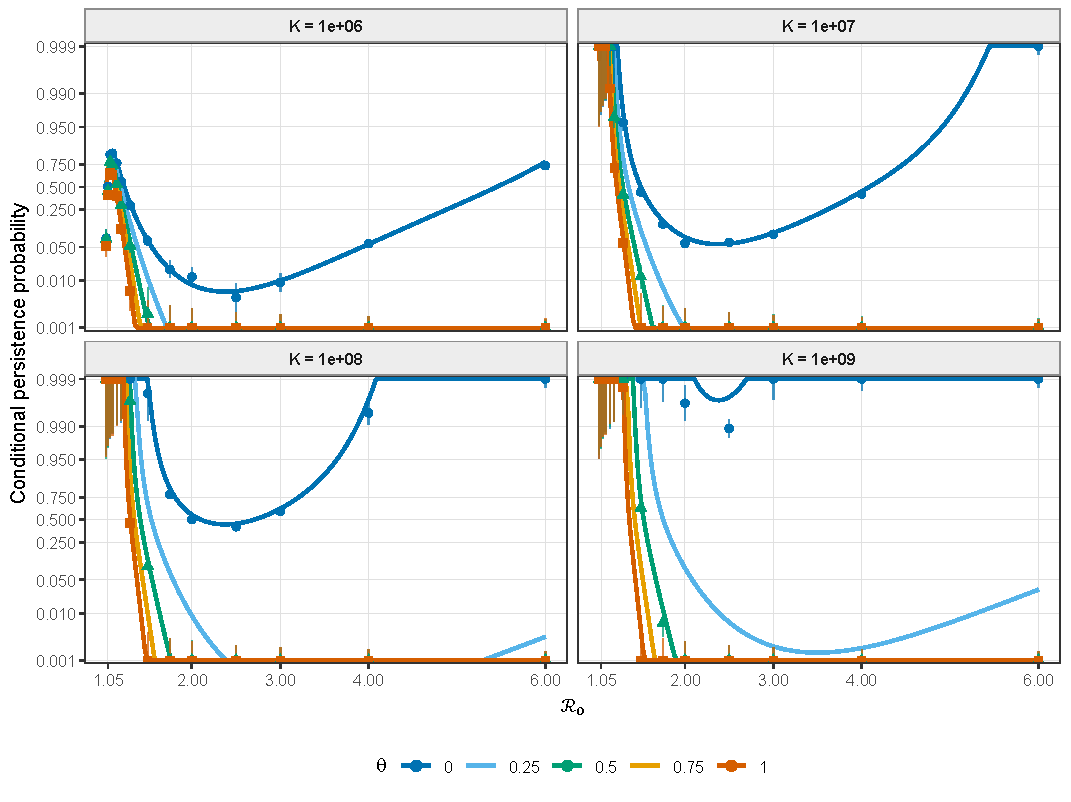
\includegraphics[width=\textwidth]{validation/figures/paper/main_persistence_validation.pdf}
\caption{Conditional persistence after epidemic establishment at \(\rhoeps=0.01\). Curves are the boundary-layer-independent prediction \cref{eq:PBI} for \(\theta=0,0.25,0.5,0.75,1\); symbols are stochastic estimates for \(\theta=0,0.5,1\), and vertical bars are 95\% Wilson intervals. The probability axis is displayed on logit coordinates so that both tails remain visible; values below 0.001 or above 0.999 are shown at those limits. The adaptive tau-leap scan used 3,000--10,000 attempted epidemics at each point. Agreement is close except at the values nearest \(\Rzero=1\), most visibly for \(K=10^6\).}
\label{fig:main-persistence}
\end{figure}

The recruitment-shape effect is systematic in the numerical sweep. For \(0<x<1\), increasing \(\theta\) reduces \(h_\theta(x)\); susceptible replenishment is consequently slower along the depleted post-wave path, the bottleneck is deeper, and conditional persistence is lower. The stochastic points follow the same ordering as the analytical curves in \cref{fig:main-persistence}. The magnitude is most visible where the parameters place the system in the transition between near-certain burnout and near-certain persistence. For example, at \((\rhoeps,\Rzero,K)=(0.01,1.5,10^8)\), the simulated conditional persistence probabilities are 0.998, 0.093, and 0 for \(\theta=0,0.5,1\), respectively; the corresponding predictions are 0.999, 0.124, and \(4.7\times10^{-4}\).

Conditional persistence itself is nonmonotone in \(\Rzero\): its boundary-independent extrema satisfy \(L=\dd\log B_{\BI}/\dd\Rzero=0\), independently of \(K\). At \(\rhoeps=0.01\), each plotted \(\theta<1\) has a near-threshold maximum followed by a minimum and, much farther out, another maximum before its eventual decline; the minima occur at \(\Rzero\simeq2.377,3.495,5.987,13.974\) for \(\theta=0,0.25,0.5,0.75\). The last minimum and the remote maxima lie beyond the range emphasized in \cref{fig:main-persistence}. For \(\theta=1\), the analytical search finds only a near-threshold maximum at \(\Rzero\simeq1.0714\); the distinct large-\(\Rzero\) behavior and the distinction from unconditional extrema are detailed in Appendix~\ref{app:numerical-diagnostics}.

\subsection{Global conditional-persistence landscape}
The same ordering persists away from the one-dimensional validation slices. Figure~\ref{fig:conditional-landscape} maps \cref{eq:PBI} over \((\Rzero,\rhoeps)\), with columns varying recruitment shape and rows separating population sizes by three orders of magnitude. Increasing \(K\) expands the high-persistence region, whereas increasing \(\theta\) contracts it and shifts its transition toward slower recruitment or larger populations. Sensitivity is strongest near the \(\theta\)-dependent transition boundary, which can move substantially: a point with near-certain persistence for one recruitment shape need not remain saturated for another. Gray cells identify where the first-order finite matching entry fails the directly derived admissibility test \(0<M_1<\Delta A_f\) in \cref{eq:admissibility}, using \(y_{\rm BL}=\sqrt{y_*/K}\). The boundary-independent formula remains mathematically defined there, but its finite-entry derivation lacks an overlap check. This diagnostic is not a theorem that every unmasked cell is quantitatively accurate; the near-critical and larger-\(\rhoeps\) limitations remain visible in \cref{fig:accuracy-map}.

\begin{figure}[t]
\centering
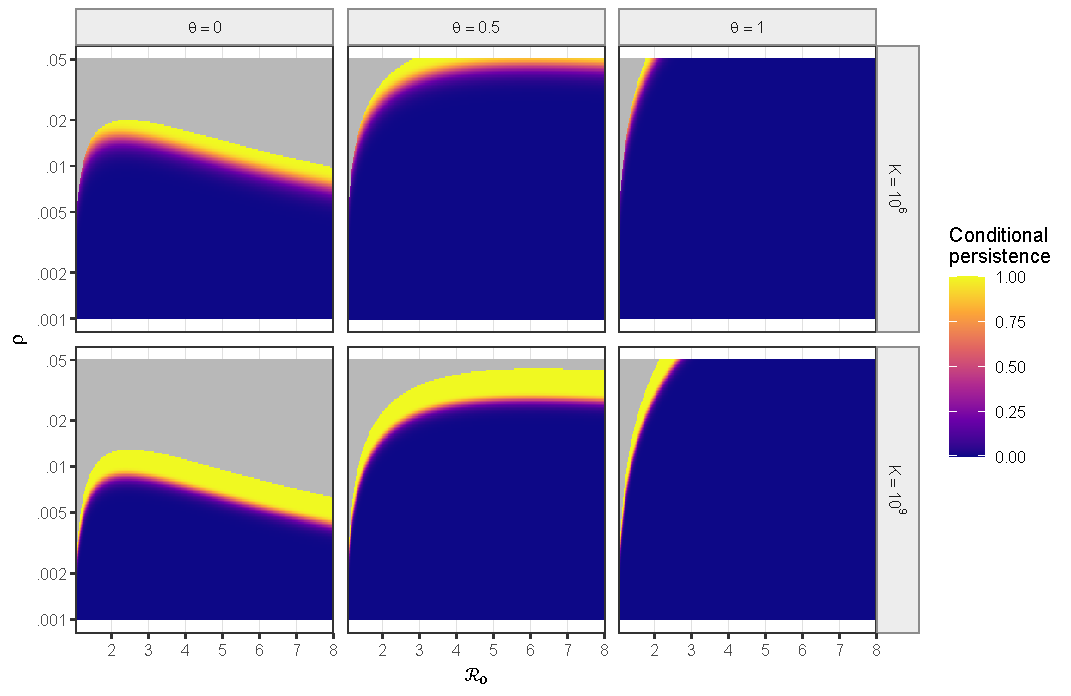
\includegraphics[width=\textwidth]{validation/figures/paper/conditional_persistence_landscape.pdf}
\caption{Boundary-layer-independent conditional persistence over transmission strength and recruitment rate. Columns show \(\theta=0,0.5,1\), and rows show \(K=10^6\) and \(10^9\). Gray cells fail the first-order finite-entry condition \(0<M_1<\Delta A_f\) at the specified matching height. This is a concrete overlap diagnostic, not a sharp accuracy boundary. Increasing recruitment nonlinearity suppresses persistence most strongly along the probability transition.}
\label{fig:conditional-landscape}
\end{figure}

\subsection{Unconditional persistence and its extrema}
To compare with the qualitative structure identified for linear recruitment by Parsons et al.\ \cite{ParsonsEtAl2024}, we include the establishment factor in \cref{eq:uncond}. The conditional post-wave probability can itself be nonmonotone in \(\Rzero\); multiplication by establishment is not, by itself, the cause of nonmonotonicity. Write \(B=B_{\BI}(\Rzero)\) and \(L=\dd\log B/\dd\Rzero\). Differentiating \cref{eq:uncond} gives the exact stationary condition for this approximation,
\begin{equation}
G(\Rzero;\rhoeps,\theta,K)
:=BL+\frac{e^B-1}{\Rzero(\Rzero-1)}=0.
\label{eq:extremumG}
\end{equation}
The second term is positive because establishment increases monotonically with \(\Rzero\). An extremum therefore requires the post-wave factor to decline sufficiently rapidly, \(L<0\), to overcome it. Recruitment shape changes this balance through \(\Cth\), the explicit \(\Rzero^{-\theta/2}\) factor in \(B\), and the action barrier \(\dAf\). The derivatives of \(\Cth\) are taken inside its finite regularized quadrature, while derivatives of \(\dAf\) are analytical; the implementation is documented in Appendix~\ref{app:numerical-diagnostics}.

Figure~\ref{fig:unconditional-structure}(a) shows unconditional persistence at \(K=10^6\), with extremum loci obtained by solving \cref{eq:extremumG}, not by differentiating a plotted grid. At the small recruitment rate \(\rhoeps=0.01\), a maximum and minimum are already present at \(\theta=0\): as \(\theta\) increases from 0 to 0.75, the maximum moves from \(\Rzero=1.182\) to 1.121, while the minimum moves from \(\Rzero=2.295\) to 12.787 and leaves the plotted \(\Rzero\leq8\) range. A minimum leaving that range is not evidence of a finite-\(\Rzero\) saddle-node. At \(\rhoeps=0.01\), \(\theta=1\), only a maximum at \(\Rzero\simeq1.1109\) is detected over \(1.01\leq\Rzero\leq80\); this slice alone does not determine behavior at other \(\rhoeps\).

The structure differs at larger \(\rhoeps\). At \(K=10^6\) and \(\rhoeps=0.02\) or 0.03, no extrema are detected at \(\theta=0\) over \(1.01\leq\Rzero\leq40\), but increasing \(\theta\) creates a maximum--minimum pair in this range. We define \(\theta_c(\rhoeps,K)\) only for this genuine pair-creation event, where \(G=G_{\Rzero}=0\), not as a generic threshold for nonmonotonicity. The critical pairs \((\mathcal R_{0,c},\theta_c)\) are \((2.1723,0.13691)\) and \((3.0619,0.32195)\), respectively; at \(\rhoeps=0.02\), changing \(K\) from \(10^5\) to \(10^7\) moves the pair from \((1.7122,0.01405)\) to \((2.7241,0.23957)\) \cref{fig:unconditional-structure}(b,c). A single extremum need not belong to a pair: for \(\theta=1\), the analytical \(G=0\) search finds only one maximum at \(\Rzero\simeq1.0528,1.1109,1.2866,1.4750\) for \(\rhoeps=0.005,0.01,0.02,0.03\), respectively, over \(1.01\leq\Rzero\leq80\). Thus the qualitative branch structure depends on \(\rhoeps\) as well as \(\theta\). Where a pair already exists at \(\theta=0\), panel (c) shows no artificial \(\theta_c=0\) point.

The representative small-\(\rhoeps\) extrema are not an artifact of the Laplace reduction. At the three minima for \(\theta=0,0.25,0.5\) and \(\rhoeps=0.01\), replacing the closed form by the finite-entry prediction with the exact Kendall integral changes conditional persistence by 1.70\%, 0.93\%, and 0.05\%, respectively. More importantly, local scans of the finite-entry, exact-Kendall unconditional probability retain both extrema just beyond the saddle-node: near \((\rhoeps,\theta)=(0.02,0.15)\), a maximum and minimum occur around \(\Rzero=1.92\) and 2.48; near \((0.03,0.34)\), they occur around 2.5 and 3.7. These checks support the qualitative branch creation, although the precise saddle-node numbers belong to the leading boundary-independent approximation.

\begin{figure}[p]
\centering
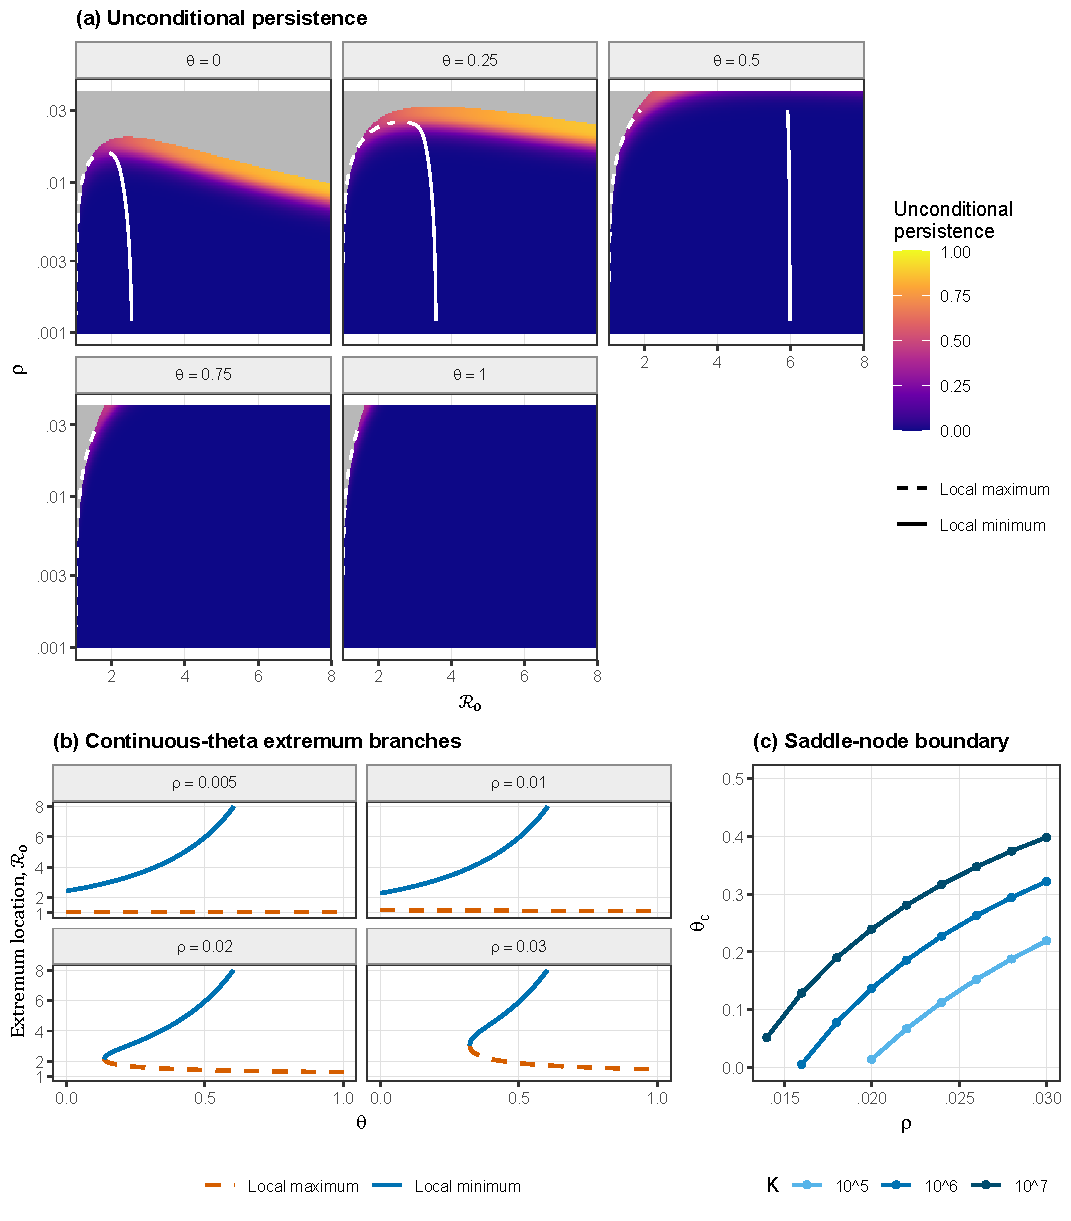
\includegraphics[width=\textwidth]{validation/figures/paper/unconditional_persistence_structure.pdf}
\caption{Analytically verified structure of unconditional persistence. (a) Landscapes at \(K=10^6\) for five recruitment shapes; white dashed and solid curves are local maxima and minima obtained from \(G=0\). Gray cells fail the first-order finite-entry condition, as in \cref{fig:conditional-landscape}. (b) Continuous extremum branches obtained by one-sided continuation of \(G=0\) in \(\theta\), initialized at \(\theta=0\) or at a verified saddle-node; branches end at the plotting boundary \(\Rzero=8\) when necessary. An empty part of (b) means no extremum within the displayed \(\Rzero\) window, not global monotonicity. (c) Genuine saddle-node pair-creation boundary obtained from \(G=G_{\Rzero}=0\). No point is plotted where a pair already exists at \(\theta=0\).}
\label{fig:unconditional-structure}
\end{figure}

\begin{figure}[H]
\centering
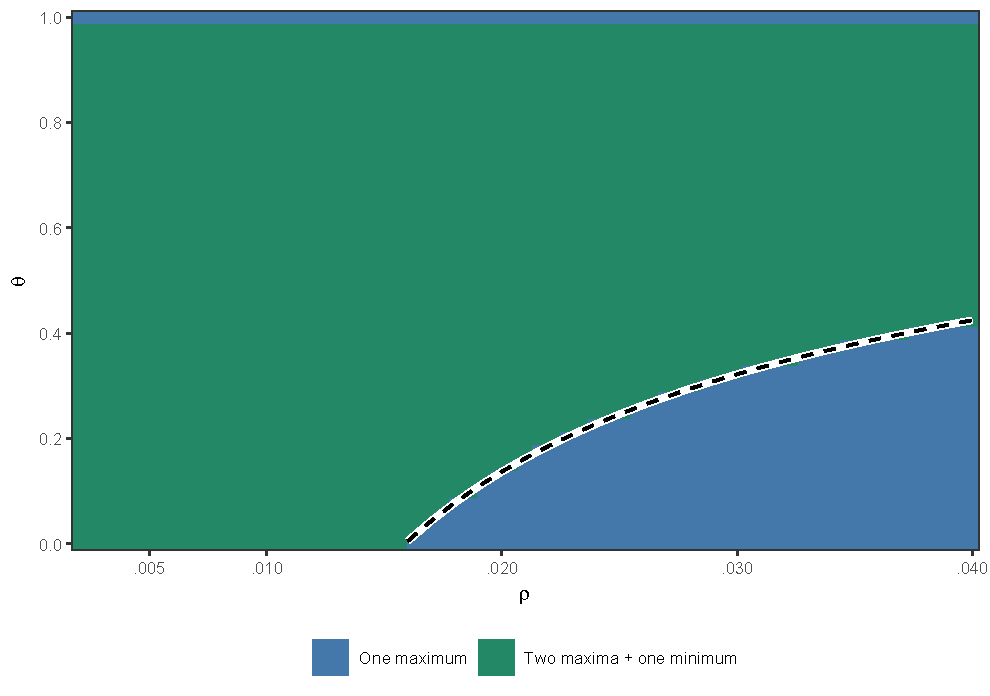
\includegraphics[width=.88\textwidth]{validation/figures/paper/unconditional_shape_map.pdf}
\caption{Global shape classification of the leading BI unconditional-persistence curve over \(\Rzero>1\), across \((\rhoeps,\theta)\) at \(K=10^6\). The observed structures are one maximum (blue, possibly far outside Figure~\ref{fig:unconditional-structure}) and two maxima separated by one minimum (green). The black dashed line is the genuine pair-creation locus \(G=G_{\Rzero}=0\), not a generic nonmonotonicity threshold. Roots are bracketed from the analytical \(G=0\) condition through \(\Rzero=300\); the far-right maximum for \(\theta<1\) is continued using the derived large-\(\Rzero\) asymptotics. This classifies the BI expression and does not validate its quantitative accuracy at extreme \(\Rzero\).}
\label{fig:unconditional-shape-map}
\end{figure}

The full-\(\Rzero\) shape classification in \cref{fig:unconditional-shape-map} is not inferred from the \(\Rzero\leq8\) display in Figure~\ref{fig:unconditional-structure}. At fixed finite \(K\), unconditional persistence vanishes both as \(\Rzero\downarrow1\) and as \(\Rzero\to\infty\), so it must have a maximum. On the mapped \((\rhoeps,\theta)\) range, the leading BI formula has either one maximum or two maxima separated by a minimum; neither a no-extremum nor a minimum-only global region occurs. The one-maximum region can nevertheless look monotone on a finite plot: at \((\rhoeps,\theta,K)=(0.02,0.005,10^6)\), \(G=0\) has no root through \(\Rzero=300\), but its large-\(\Rzero\) continuation gives a maximum near \(\Rzero=3.2\times10^6\). For \(\theta<1\), such far-right maxima are retained in the global count, while an additional finite maximum--minimum pair is not automatic. At \(\theta=1\), only one maximum is found throughout \(0.002\leq\rhoeps\leq0.04\); an extended analytical-root scan over \(0.001\leq\rhoeps\leq1\) likewise detects no additional pair or fixed-\(\theta=1\) saddle-node. The dashed \(\theta_c\) curve marks creation of the additional maximum--minimum pair, not the onset of nonmonotonicity. Increasing \(K\) shifts this pair-creation boundary to larger \(\theta\), as the companion maps in Appendix~\ref{app:numerical-diagnostics} show.

\subsection{Validity map and regions of reduced accuracy}
Figure~\ref{fig:accuracy-map} localizes the discrepancy between theory and stochastic simulation at the representative size \(K=3\times10^4\). Most well-separated points have small absolute probability error. Larger errors concentrate at faster recruitment and toward \(\Rzero\downarrow1\), where the fixed-\(\Rzero\) asymptotics lose separation. Small neutral crosses mark the directly computed failure of \(0<M_1<\dAf\), not a fitted or purportedly exact accuracy threshold. Across the full stochastic cache, the mean absolute error rises from 0.011 at \(\rhoeps=0.01\) to 0.018, 0.043, and 0.096 at \(\rhoeps=0.02,0.05,0.10\). At the two larger values the leading closed form commonly underestimates persistence in the transition region. The earlier curve \(\Rzero=e^{2\rhoeps}\) was only a heuristic proxy for \(\Rzero-1=O(\rhoeps)\); it is no longer used as a validity boundary.

\begin{figure}[t]
\centering
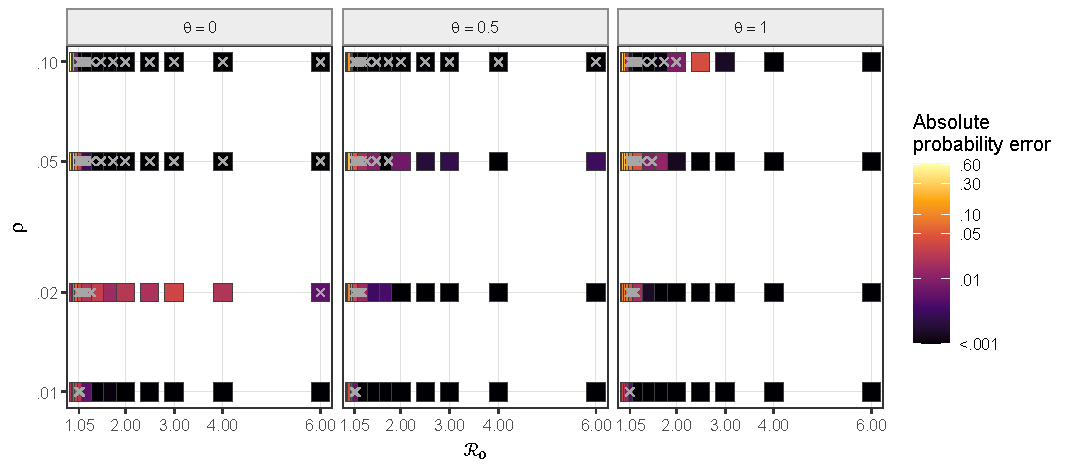
\includegraphics[width=\textwidth]{validation/figures/paper/stochastic_error_validity_map.pdf}
\caption{Absolute error of the boundary-layer-independent conditional-persistence prediction against stochastic simulation at \(K=3\times10^4\). Square color gives absolute probability error on a logarithmic scale. Small neutral crosses mark points where the first-order finite matching entry is inadmissible, \(M_1\notin(0,\dAf)\). This is an overlap diagnostic rather than a sharp error guarantee.}
\label{fig:accuracy-map}
\end{figure}

The conspicuous near-critical exception in \cref{fig:main-persistence} has the same interpretation. At \(K=10^6\) and \(\Rzero=1.03\), the theory predicts conditional persistence probabilities of 0.46--0.48, whereas the simulations give 0.05--0.08. The discrepancy occurs for all three simulated values of \(\theta\), despite the large population size, and therefore does not have the signature of a recruitment-shape or ordinary finite-\(K\) effect. Rather, \(\Rzero-1\) is then comparable to the recruitment scale, so the epidemic excursion, post-wave relaxation, and stochastic bottleneck are no longer separated. The prediction has recovered by \(\Rzero=1.075\)--1.10 in the same panel.

\enlargethispage{2\baselineskip}
The ODE and Kendall diagnostics localize the remaining error (Appendix~\ref{app:numerical-diagnostics}). On points for which a finite matching entry exists, replacing the numerical ODE entry by the second-order asymptotic entry changes conditional persistence by only 0.0009--0.0015 on average over \(\rhoeps=0.02\)--0.10. The errors from reducing the ODE-plus-exact-Kendall reference to the boundary-independent closed form, and from applying Laplace's method, are an order of magnitude larger. Thus second-order matching is working as intended where an overlap exists; the conspicuous failures arise mainly when that overlap disappears or the saddle approximation is no longer sharply separated. For high-accuracy calculations near this edge, the finite-entry prediction with the exact one-dimensional Kendall integral should be retained.

\clearpage
\section{Discussion}
\label{sec:discussion}
The main conclusion is that the asymptotic burnout framework developed for linear susceptible replenishment extends quantitatively to the broader family \(\hth(x)=(1-x)x^\theta\). The leading first-wave epidemic trajectory is shared across this family, while the recruitment law enters through the post-wave corrections that determine the low-prevalence trough and the subsequent extinction calculation. In the well-separated regime the resulting closed-form persistence probability follows the full stochastic simulations closely across population size, transmission strength, and recruitment shape.

Within this family, the pointwise effect of recruitment shape has a clear direction. Increasing \(\theta\) suppresses recruitment whenever susceptibles have been depleted below carrying capacity, deepens the post-wave bottleneck, and reduces conditional persistence at fixed \((\Rzero,\rhoeps,K)\). The practical size of this effect is strongly parameter dependent: it is negligible when every recruitment law already predicts almost certain burnout or persistence, but can markedly displace the transition region in \((\Rzero,\rhoeps,K)\). This dependence is a post-wave effect that coexists with the \(\theta\)-independent leading geometry of the first epidemic wave.

The global effect is richer than this pointwise ordering. Conditional post-wave persistence may already be nonmonotone in \(\Rzero\), whereas the establishment factor \(1-1/\Rzero\) is strictly increasing. The analytical condition \cref{eq:extremumG} shows that extrema of their product occur only when the post-wave contribution decreases rapidly enough to outweigh increasing establishment. At fixed finite \(K\), the unconditional BI probability returns to zero at large \(\Rzero\): algebraically for \(\theta<1\), because \(\Cth\propto\Rzero^{-1}\), and exponentially for \(\theta=1\), because the action grows linearly. Thus \(\theta=1\) is a qualitative boundary in decay rate, not in the limiting probability. At \(\rhoeps=0.01\), increasing \(\theta\) moves the finite-region maximum and minimum in opposite directions; a minimum leaving a plotting window is not evidence of annihilation. At larger \(\rhoeps\), \(G=G_{\Rzero}=0\) confirms creation of an additional pair through a genuine saddle-node. The shape map shows that this pair is not automatic for \(\theta<1\), and that its creation value \(\theta_c\) depends on \((\rhoeps,K)\) rather than marking a generic onset of nonmonotonicity.

This extension is biologically relevant because the form of susceptible recruitment depends on the host population being modeled. Linear replenishment is a convenient approximation for demographic turnover in many standard human-disease SIR models, whereas ecological host populations may exhibit stronger density dependence as population size approaches a carrying capacity. The present family provides a simple interpolation between these cases. The analysis therefore makes explicit that assumptions about host demography can affect post-wave persistence even when the leading first epidemic wave is unchanged.

Several limitations delimit the present theory. First, the asymptotic construction assumes slow susceptible recruitment, \(\rhoeps\to0\), with fixed \(\Rzero>1\). The simulations show directly that a different near-critical analysis is required when \(\Rzero-1\) approaches the recruitment scale. Second, the deterministic entry state neglects finite-population fluctuations, including variability in the susceptible state inherited from the first wave; these can matter at smaller \(K\). Third, the time-inhomogeneous branching-process approximation is designed for the low-prevalence phase and is not intended to replace full stochastic simulation of the complete epidemic. Finally, \(\hth(x)=(1-x)x^\theta\) is still a restricted one-parameter family and does not represent all biologically plausible recruitment mechanisms.

These limitations suggest several directions for future work. A natural first extension is to replace the one-parameter family by a more general recruitment function \(h(x)\) and determine which parts of the matching and burnout calculation depend only on local properties of \(h\) and which require its global form. Broader transmission structures are distinct because they may alter the leading epidemic geometry itself. Other extensions could incorporate seasonal forcing, spatial or host heterogeneity, or a stochastic treatment of the entry state. A further empirical direction would be to estimate recruitment functions from host-demographic data and quantify how uncertainty in those functions propagates into predicted burnout probabilities.

Overall, generalized susceptible recruitment changes the post-wave trajectory without changing the leading first-wave orbit. Extending the existing burnout approximation to this setting connects host-demographic assumptions to both the magnitude and the nonmonotone structure of post-wave persistence. When a valid finite entry and deterministic-to-stochastic overlap remain, the exact one-dimensional Kendall integral can replace an inaccurate Laplace or boundary-independent reduction; when that overlap or scale separation fails, full stochastic simulation or a different asymptotic treatment is needed.

\appendix
\section{Regularized second-order matching constant \(\Dth\)}
\label{app:Dtheta}
This appendix records the production-level regularization underlying \cref{eq:X2asymp}. Let
\[
s=x-\xf,\qquad
f_1=F'(\xf)=\frac{\delta}{\Rzero\xf},
\qquad
f_2=F''(\xf)=-\frac{1}{\Rzero\xf^2}.
\]
Writing \(G_\theta=\Rzero Y_1\), define
\[
\alpha=\frac{h_f}{\Rzero\xf},
\qquad
\beta=\alpha\log\frac{f_1}{\Cth}.
\]
The first-order local expansion takes the form
\begin{equation}
Y_1(\xf+s)=\alpha\log s+\beta+p_0s+O(s^2),
\label{eq:Y1localapp}
\end{equation}
where
\begin{equation}
p_0=\frac{2\delta\xf h_f'-(1+2\delta)h_f}
{2\Rzero\delta\xf^2}.
\label{eq:p0}
\end{equation}
Define
\begin{equation}
A_{-1}=\frac{h_f/\xf-c}{\delta^2},
\qquad
B_0=\beta-\alpha,
\qquad
B_1=-\frac{h_f}{2\Rzero\delta\xf^2}.
\label{eq:ABdefs}
\end{equation}
The singular part of \(Y_2'\) is
\begin{equation}
q_{2,\rm sing}(s)=
-\frac{a\alpha\log s+aB_0}{s^2}
+\frac{A_{-1}\alpha\log s+A_{-1}B_0-aB_1}{s}.
\label{eq:q2sing}
\end{equation}
A corresponding primitive is
\begin{equation}
P_2(s)=
\frac{a\alpha\log s+a\beta}{s}
+\frac{A_{-1}\alpha}{2}\log^2s
+(A_{-1}B_0-aB_1)\log s.
\label{eq:P2}
\end{equation}
Let \(q_2(x)\) denote the right-hand side of \cref{eq:Y2prime} and define
\[
q_{2,\rm reg}(x)=q_2(x)-q_{2,\rm sing}(x-\xf).
\]
Then \(q_{2,\rm reg}(x)=O(\log(x-\xf))\) is integrable at \(\xf\), and
\begin{equation}
K_2=-P_2(1-\xf)-\int_{\xf}^{1}q_{2,\rm reg}(u)\dd u.
\label{eq:K2}
\end{equation}
The constant term in the numerator of \cref{eq:X2general} is
\begin{equation}
N_{20}=K_2+
\frac{\alpha\beta f_2}{f_1^2}
-\frac{(\alpha+\beta)p_0}{f_1}
+\frac{f_2\beta^2}{2f_1^2}.
\label{eq:N20}
\end{equation}
The regularized second-order matching constant is therefore
\begin{equation}
\Dth=-\frac{N_{20}}{f_1}-\kappa\frac{\beta^2}{\alpha^2}.
\label{eq:DthetaApp}
\end{equation}
This formula requires only finite regularized quadrature and local algebra. No small-\(y\) extrapolation is required.

\section{Laplace correction}
\label{app:laplace}
Let \(z=X-\xs\), \(h_*=\hth(\xs)\), and \(\lambda=\Rzero/h_*>0\). Since
\[
\Ath'(\xs+z)=-\frac{\Rzero z}{\hth(\xs+z)},
\]
the required derivatives at the saddle are
\begin{align}
\Ath'''(\xs)&=\frac{2\Rzero h_*'}{h_*^2},\\
\Ath''''(\xs)&=-\frac{6\Rzero(h_*')^2}{h_*^3}
+\frac{3\Rzero h_*''}{h_*^2}.
\end{align}
Applying Gaussian averaging to the amplitude \(1/\hth\) after \(z=\sqrt{\rhoeps}\,t\) gives the relative correction \(1+\rhoeps c_L+O(\rhoeps^2)\), with \(c_L\) given by \cref{eq:cL}. For the recruitment family \cref{eq:hth},
\begin{align}
\hth'(x)&=x^{\theta-1}\{\theta-(\theta+1)x\},\\
\hth''(x)&=\theta x^{\theta-2}\{(\theta-1)-(\theta+1)x\}.
\end{align}
In particular, at \(\theta=0\), \(c_L=1/[12(\Rzero-1)]\).

\section{Implementation and diagnostic quantities}
\label{app:numerical-diagnostics}
\subsection{Conditional extrema and the large-\(\Rzero\) limit}
For \(P_c=1-e^{-B_{\BI}}\), direct differentiation gives
\begin{equation}
\frac{\dd P_c}{\dd\Rzero}=e^{-B_{\BI}}B_{\BI}L,
\qquad
L=(\log\Cth)'+\frac{1}{2(\Rzero-1)}
-\frac{\theta}{2\Rzero}-\frac{\dAf'}{\rhoeps}.
\label{eq:conditionalL}
\end{equation}
Thus the sign changes of \(L\), rather than differences of sampled probabilities, classify conditional extrema. The factor \(K\) enters \(\log B_{\BI}\) only through \(\log K\), so every BI conditional-extremum location is exactly independent of \(K\). This differs from the unconditional condition \(G=0\) in \cref{eq:extremumG}, which contains \(B\) and hence depends on \(K\).

At \(\rhoeps=0.01\), analytical-derivative root searches give the successive maximum, minimum, and remote maximum at \(\Rzero\simeq(1.093717,2.377372,101.670522)\) for \(\theta=0\), \((1.086160,3.494824,413.8)\) for \(\theta=0.25\), \((1.080250,5.986866,7.904\times10^3)\) for \(\theta=0.5\), and \((1.075435,13.973974,6.988\times10^7)\) for \(\theta=0.75\). The last three remote-maxima values use the large-\(\Rzero\) continuation below, avoiding underflow in \(x_f\); the near-threshold extrema and the \(\theta=0\) remote maximum use the full regularized derivative. For \(\theta=1\), the sole detected zero is a maximum at \(\Rzero=1.071397\); no later minimum is detected on the numerically accessible finite range. These are properties of the leading BI formula, not additional stochastic-validation claims.

To determine the eventual sign without extrapolating a finite plot, use \(x_f=-W_0(-\Rzero e^{-\Rzero})/\Rzero\sim e^{-\Rzero}\). For each fixed \(0\leq\theta<1\), setting \(u=x_f e^s\) in the regularized quadrature isolates the \(-\Rzero\) outer contribution. The remaining lower-end integral tends to
\[
c_\theta=\int_0^\infty\left\{\frac{e^{-(1-\theta)s}}{s}
-\frac{1}{e^s-1}\right\}\dd s
=-\gamma_{\rm E}-\log(1-\theta),
\]
where the difference is finite at \(s=0\). Splitting the transformed integral into a fixed lower-end interval and its exponentially decaying tail, then differentiating under the same split, gives \(J_\theta/\tilde a=-\Rzero+c_\theta+o(1)\), \(\log\Cth=-\log\Rzero+c_\theta+o(1)\), and \((\log\Cth)'=-1/\Rzero+o(1/\Rzero)\). Meanwhile \(\dAf'=-1/[(2-\theta)\Rzero^{2-\theta}]+O(\Rzero^{-(3-\theta)})+O(e^{-(1-\theta)\Rzero})\). Consequently,
\begin{equation}
L=-\frac{1+\theta}{2\Rzero}
+\frac{1}{\rhoeps(2-\theta)\Rzero^{2-\theta}}
+o(\Rzero^{-1})<0
\qquad(0\leq\theta<1,\ \Rzero\to\infty).
\label{eq:LlargeSublinear}
\end{equation}
The remote maximum follows from balancing the two displayed terms, giving \(\Rzero\sim[2/\{\rhoeps(2-\theta)(1+\theta)\}]^{1/(1-\theta)}\) when that root is asymptotically large. At \(\theta=1\), the amplitude instead approaches \(e^{-1}\), with \((\log C_1)'=O(\Rzero^{-2})\), and \(\dAf'=1-1/\Rzero+O(\Rzero^{-2})\); hence \(L=-1/\rhoeps+O(\Rzero^{-1})<0\). The large-\(\Rzero\) decline therefore holds at both endpoints, although the action term changes qualitatively at \(\theta=1\).

Writing \(\delta=1-\theta\downarrow0\), the minimum occurs in the crossover where \(x_f^\delta\sim e^{-\delta\Rzero}\) competes with \(\int_0^{1/\Rzero}x^\delta/(1-x)\,\dd x\sim\Rzero^{-1-\delta}/(1+\delta)\). The amplitude derivative contributes at order \(1/\Rzero\), not at order one, so this balance yields \(\delta\Rzero\sim\log\Rzero\) and
\begin{equation}
\mathcal R_{0,\min}(\theta)\sim\frac{\log[1/(1-\theta)]}{1-\theta}
\qquad(\theta\uparrow1)
\label{eq:conditionalMinScaling}
\end{equation}
at leading logarithmic order. Numerical continuation gives minima at \(\Rzero\simeq42.10,97.23,290.75\) for \(\theta=0.9,0.95,0.98\), respectively; the minimum escapes to infinity rather than meeting the near-threshold maximum at finite \(\Rzero\). The remote maximum diverges still faster. The asymptotic statements establish eventual signs and escape scales; the finite-range root count is a numerical observation, not a global root-count theorem.

\subsection{Derivative implementation and diagnostic quantities}
For the extremum calculation, differentiating the implicit final-size equation gives
\begin{equation}
x_f'=\frac{x_f(x_f-1)}{1-\Rzero x_f}.
\end{equation}
The action barrier is differentiated analytically rather than by differencing its values:
\begin{align}
\dAf'&=x_f^{1-\theta}-\int_{x_f}^{1/\Rzero}\frac{x^{1-\theta}}{1-x}\dd x,\\
\dAf''&=\frac{\Rzero^{\theta-2}}{\Rzero-1}
-\frac{x_f^{1-\theta}[(1-\theta)+\theta x_f]}{1-\Rzero x_f}.
\end{align}
The matching amplitude \(\Cth\) is a fully specified semi-analytical quantity, not a fitted coefficient. Writing \(x_*=1/\Rzero\), \(\tilde a=(1-x_f)x_f^{\theta-1}\), and
\begin{equation}
q(u;\Rzero,\theta)=\frac{(x_*-u)h_\theta(u)}{u^2F(u;\Rzero)}
-\frac{\tilde a}{u-x_f},
\end{equation}
its regularized quadrature is \(J_\theta=\int_{x_f}^{1}q(u;\Rzero,\theta)\dd u\) and
\begin{equation}
\log\Cth=\log(1-x_f)+\log(x_*-x_f)-\log x_f+\frac{J_\theta}{\tilde a}.
\end{equation}
For the directly evaluated \(\Rzero\) range, set \(u=x_f e^s\), \(0<s<-\log x_f\), and then map \(s=t(-\log x_f)\) to fixed limits \(0<t<1\). The integrand for \(J_\theta/\tilde a\) becomes
\[
\frac{(x_*-u)(1-u)e^{(\theta-1)s}}{(1-x_f)F(u;\Rzero)}
-\frac{e^s}{e^s-1},
\qquad F(x_f e^s;\Rzero)=x_f(1-e^s)+\frac{s}{\Rzero},
\]
whose apparent lower-end singularities cancel. The implementation propagates the first two \(\Rzero\)-derivatives through this fixed-limits regularized quadrature and through \(\log\Cth\); finite differences are used only to check the result.

In particular,
\begin{align}
L&=(\log\Cth)'+\frac{1}{2(\Rzero-1)}-\frac{\theta}{2\Rzero}-\frac{\dAf'}{\rhoeps},\\
L'&=(\log\Cth)''-\frac{1}{2(\Rzero-1)^2}+\frac{\theta}{2\Rzero^2}-\frac{\dAf''}{\rhoeps},
\end{align}
and the saddle-node test uses
\begin{equation}
G_{\Rzero}=B(L^2+L')-\frac{(2\Rzero-1)(e^B-1)}{\Rzero^2(\Rzero-1)^2}
+\frac{e^BBL}{\Rzero(\Rzero-1)}.
\end{equation}
The numerical solver evaluates \(G/B\) and \(G_{\Rzero}/B\) to avoid underflow when \(B\) is very small; these have the same simultaneous zeros as the unscaled equations for \(B>0\). At the reported critical pairs the largest scaled residual is below \(2\times10^{-11}\). Quadrature-level derivatives agree with centered finite-difference diagnostics at representative points, without using finite differences to locate extrema or saddle-nodes.

\subsection{Global unconditional-shape classification}
Let \(\varepsilon=\Rzero-1\downarrow0\). The final-size roots coalesce as \(x_f=1-2\varepsilon+O(\varepsilon^2)\) and \(x_*=1-\varepsilon+O(\varepsilon^2)\). Rescaling the regularized amplitude integral across this shrinking interval gives \(J_\theta/\tilde a\to-2\), uniformly for fixed \(0\leq\theta\leq1\), and hence \(\Cth\sim2e^{-2}\varepsilon^2\). Since \(\dAf=O(\varepsilon)\), the BI exponent and unconditional persistence obey
\[
B_{\BI}\sim2e^{-2}K\sqrt{\frac{\rhoeps}{2\pi}}\,\varepsilon^{5/2},
\qquad
P_{\rm persist,uncond}\sim2e^{-2}K\sqrt{\frac{\rhoeps}{2\pi}}\,\varepsilon^{7/2}.
\]
Thus the BI curve starts at zero and initially increases. These are endpoint properties of the BI expression, whose finite-\(\rhoeps\) accuracy close to \(\Rzero=1\) remains nonuniform.

At the opposite endpoint, the amplitude asymptotic derived above is decisive. For fixed \(0\leq\theta<1\), writing \(\delta=1-\theta\), the action satisfies \(\dAf\sim[\delta(1+\delta)\Rzero^\delta]^{-1}\to0\), while \(\Cth\sim e^{-\gamma_{\rm E}}/(\delta\Rzero)\). Therefore
\begin{equation}
B_{\BI}\sim\frac{K e^{-\gamma_{\rm E}}}{1-\theta}
\sqrt{\frac{\rhoeps}{2\pi}}\,
\Rzero^{-(1+\theta)/2},
\qquad
P_{\rm persist,uncond}\sim B_{\BI}\to0.
\label{eq:uncondLargeSublinear}
\end{equation}
In particular, the far-tail derivative is negative, not positive: dropping the \(\Cth\propto\Rzero^{-1}\) factor would give the wrong endpoint conclusion. For \(\theta=1\), \(\Cth\to e^{-1}\) but \(\dAf'=1-1/\Rzero+O(\Rzero^{-2})\), so \(\dAf=\Rzero-\log\Rzero+O(1)\) and \(B_{\BI}\to0\) exponentially. The \(\theta=1\) endpoint is thus qualitatively different in decay rate, but not in the limiting value \(P_{\rm persist,uncond}(\infty)=0\). Together with the near-threshold rise, both endpoint laws require at least one local maximum; a no-extremum or minimum-only global shape is excluded.

For \cref{fig:unconditional-shape-map}, the analytical \(G/B\) condition was bracketed on a dense grid spanning \(1.001\leq\Rzero\leq300\), with each root refined and classified by the sign of \(G_{\Rzero}\). The \(\theta\)-grid reaches 0.975 before the separate endpoint \(\theta=1\); the tracked finite minimum remains below \(\Rzero=300\) on this grid. For \(\theta<1\), a further maximum was located by solving the large-\(\Rzero\) continuation obtained from \cref{eq:uncondLargeSublinear} and the corresponding action expansion. Thus zero finite-window roots correspond to one remote maximum, while a finite maximum--minimum sequence is followed by a remote second maximum. This tail continuation is essential for shape counting but can lie far beyond the regime of quantitative stochastic validation. No extra finite-window roots or minimum-only cases were found on the mapped grid.

Figure~\ref{fig:supp-shape-map} compares the same classification at three population sizes. At \(\rhoeps=0.02\), the pair-creation value moves from \(\theta_c\simeq0.0141\) at \(K=10^5\) to 0.1369 at \(10^6\) and 0.2396 at \(10^7\). Increasing \(K\) therefore enlarges the one-maximum region and contracts the region with the additional maximum--minimum pair; the dependence is not merely a shift of plotted root locations.

\begin{figure}[H]
\centering
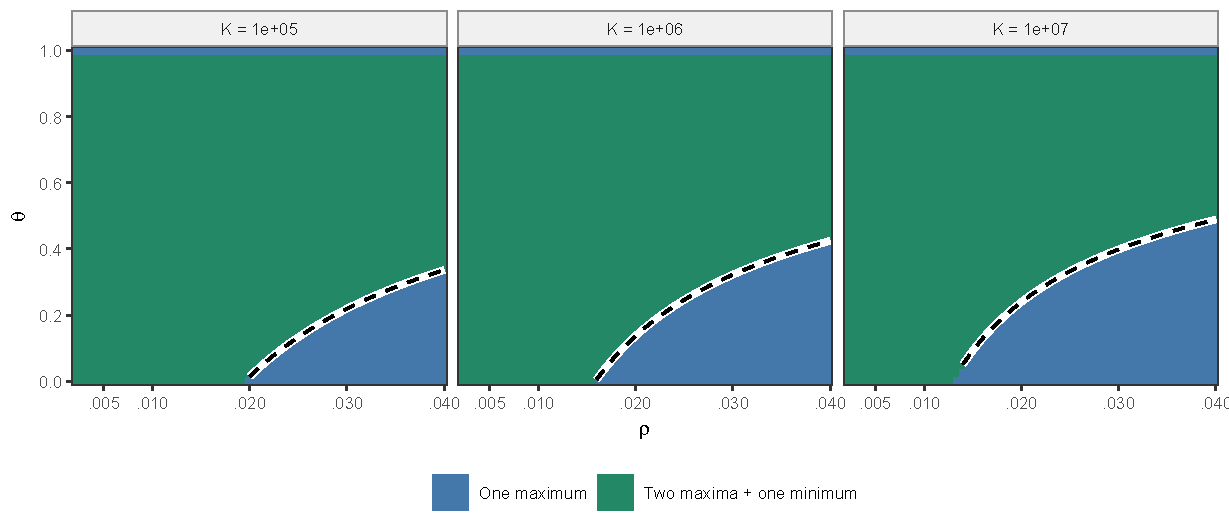
\includegraphics[width=\textwidth]{validation/figures/paper/unconditional_shape_map_K_comparison.pdf}
\caption{Unconditional-persistence shape maps for \(K=10^5,10^6,10^7\), classified as in \cref{fig:unconditional-shape-map}. The dashed line in each panel is the genuine \(G=G_{\Rzero}=0\) pair-creation locus. Higher \(K\) moves this boundary toward larger \(\theta\); the endpoint \(\theta=1\) remains a one-maximum curve over the displayed \(\rhoeps\) range.}
\label{fig:supp-shape-map}
\end{figure}

Figure~\ref{fig:supp-diagnostics} summarizes the numerical error isolation. Panel (a) compares the boundary-layer-independent prediction with stochastic simulation. Panel (b) compares approximation layers where a finite entry exists, using the numerical ODE entry and exact Kendall integral as the reference. The small second-order entry error shows that matching is not the principal source of the visible discrepancies; the larger closed-form and Laplace differences reflect weakening scale separation.

\begin{figure}[H]
\centering
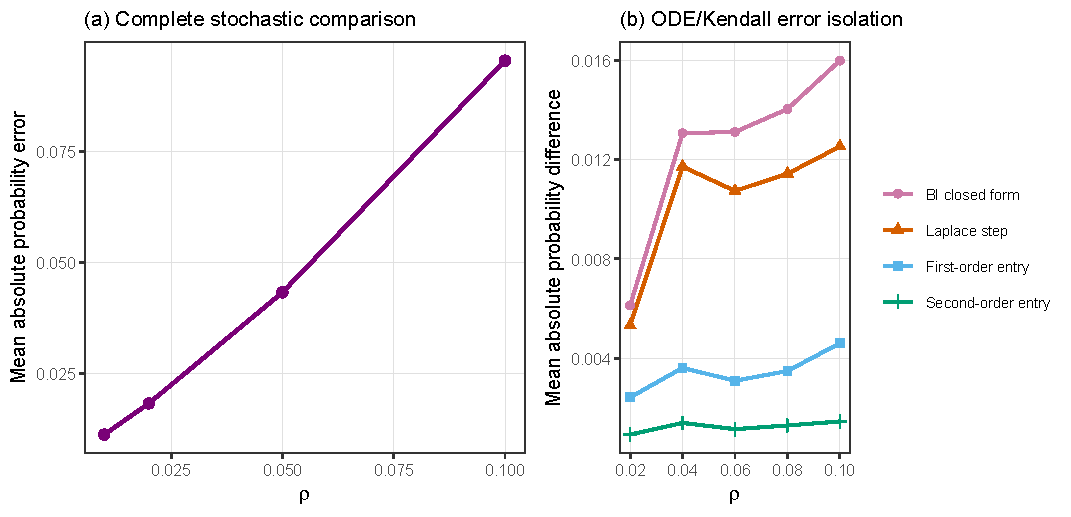
\includegraphics[width=\textwidth]{validation/figures/paper/accuracy_diagnostics_supplement.pdf}
\caption{Supplementary accuracy diagnostics. (a) Mean absolute error of the boundary-layer-independent conditional persistence probability against all cached stochastic estimates at each \(\rhoeps\). (b) Mean absolute probability differences on finite-entry points of the ODE scan. ``BI closed form'' compares \cref{eq:PBI} with the numerical-ODE-entry, exact-Kendall reference; ``Laplace step'' replaces exact Kendall by its saddle approximation while retaining the ODE entry; the other curves replace the ODE entry by the first- or second-order asymptotic entry while retaining exact Kendall. The second-order entry contribution remains near \(10^{-3}\), whereas loss in the closed-form and Laplace reductions is larger.}
\label{fig:supp-diagnostics}
\end{figure}

A numerical implementation should retain diagnostics that identify which approximation layer is failing. Useful quantities include
\[
\frac{y_{\min}^{\rm ODE}}{\yin},
\qquad
\frac{x_{\rm in}^{(1)}-x_{\rm in}^{\rm ODE}}{x_{\rm in}^{\rm ODE}},
\qquad
\frac{x_{\rm in}^{(2)}-x_{\rm in}^{\rm ODE}}{x_{\rm in}^{\rm ODE}},
\]
together with the action errors
\[
\Delta\Lambda_j=
\frac{\Ath(x_{\rm in}^{\rm ODE})-\Ath(x_{\rm in}^{(j)})}{\rhoeps},
\qquad j=1,2,
\]
and separate exact-Kendall and Laplace burnout exponents. The regularized quadrature defining \(\Dth\) should also be tested for endpoint-treatment and numerical-precision sensitivity.

For repeated parameter studies, a natural computational decomposition is:
\begin{enumerate}[leftmargin=2em]
\item for each \((\Rzero,\theta)\), compute \(\xf\), \(\Cth\), and \(\Dth\);
\item for each \((\rhoeps,K)\), compute \(y_*\) and the chosen finite matching height if the finite-boundary route is used;
\item solve \cref{eq:actionentry} for first- or second-order entry and evaluate the exact one-dimensional Kendall integral for the high-accuracy finite-boundary prediction;
\item evaluate \cref{eq:BBI} or \cref{eq:Bnext} for a boundary-layer-independent closed form;
\item record no-entry status, action size, and the difference between first- and second-order predictions as validity diagnostics.
\end{enumerate}

\begin{thebibliography}{9}
\bibitem{ParsonsEarn2024}
T. L. Parsons and D. J. D. Earn,
\newblock Uniform Asymptotic Approximations for the Phase Plane Trajectories of the SIR Model with Vital Dynamics,
\newblock \emph{SIAM Journal on Applied Mathematics} 84(4), 1580--1608 (2024).

\bibitem{ParsonsEtAl2024}
T. L. Parsons, B. M. Bolker, J. Dushoff, and D. J. D. Earn,
\newblock The probability of epidemic burnout in the stochastic SIR model with vital dynamics,
\newblock \emph{Proceedings of the National Academy of Sciences} 121(5), e2313708120 (2024).
\end{thebibliography}

\end{document}
